% Options for packages loaded elsewhere
\PassOptionsToPackage{unicode}{hyperref}
\PassOptionsToPackage{hyphens}{url}
%
\documentclass[
  11pt,
]{article}
\usepackage{amsmath,amssymb}
\usepackage{iftex}
\ifPDFTeX
  \usepackage[T1]{fontenc}
  \usepackage[utf8]{inputenc}
  \usepackage{textcomp} % provide euro and other symbols
\else % if luatex or xetex
  \usepackage{unicode-math} % this also loads fontspec
  \defaultfontfeatures{Scale=MatchLowercase}
  \defaultfontfeatures[\rmfamily]{Ligatures=TeX,Scale=1}
\fi
\usepackage{lmodern}
\ifPDFTeX\else
  % xetex/luatex font selection
\fi
% Use upquote if available, for straight quotes in verbatim environments
\IfFileExists{upquote.sty}{\usepackage{upquote}}{}
\IfFileExists{microtype.sty}{% use microtype if available
  \usepackage[]{microtype}
  \UseMicrotypeSet[protrusion]{basicmath} % disable protrusion for tt fonts
}{}
\makeatletter
\@ifundefined{KOMAClassName}{% if non-KOMA class
  \IfFileExists{parskip.sty}{%
    \usepackage{parskip}
  }{% else
    \setlength{\parindent}{0pt}
    \setlength{\parskip}{6pt plus 2pt minus 1pt}}
}{% if KOMA class
  \KOMAoptions{parskip=half}}
\makeatother
\usepackage{xcolor}
\usepackage[margin=1in]{geometry}
\usepackage{color}
\usepackage{fancyvrb}
\newcommand{\VerbBar}{|}
\newcommand{\VERB}{\Verb[commandchars=\\\{\}]}
\DefineVerbatimEnvironment{Highlighting}{Verbatim}{commandchars=\\\{\}}
% Add ',fontsize=\small' for more characters per line
\usepackage{framed}
\definecolor{shadecolor}{RGB}{248,248,248}
\newenvironment{Shaded}{\begin{snugshade}}{\end{snugshade}}
\newcommand{\AlertTok}[1]{\textcolor[rgb]{0.94,0.16,0.16}{#1}}
\newcommand{\AnnotationTok}[1]{\textcolor[rgb]{0.56,0.35,0.01}{\textbf{\textit{#1}}}}
\newcommand{\AttributeTok}[1]{\textcolor[rgb]{0.13,0.29,0.53}{#1}}
\newcommand{\BaseNTok}[1]{\textcolor[rgb]{0.00,0.00,0.81}{#1}}
\newcommand{\BuiltInTok}[1]{#1}
\newcommand{\CharTok}[1]{\textcolor[rgb]{0.31,0.60,0.02}{#1}}
\newcommand{\CommentTok}[1]{\textcolor[rgb]{0.56,0.35,0.01}{\textit{#1}}}
\newcommand{\CommentVarTok}[1]{\textcolor[rgb]{0.56,0.35,0.01}{\textbf{\textit{#1}}}}
\newcommand{\ConstantTok}[1]{\textcolor[rgb]{0.56,0.35,0.01}{#1}}
\newcommand{\ControlFlowTok}[1]{\textcolor[rgb]{0.13,0.29,0.53}{\textbf{#1}}}
\newcommand{\DataTypeTok}[1]{\textcolor[rgb]{0.13,0.29,0.53}{#1}}
\newcommand{\DecValTok}[1]{\textcolor[rgb]{0.00,0.00,0.81}{#1}}
\newcommand{\DocumentationTok}[1]{\textcolor[rgb]{0.56,0.35,0.01}{\textbf{\textit{#1}}}}
\newcommand{\ErrorTok}[1]{\textcolor[rgb]{0.64,0.00,0.00}{\textbf{#1}}}
\newcommand{\ExtensionTok}[1]{#1}
\newcommand{\FloatTok}[1]{\textcolor[rgb]{0.00,0.00,0.81}{#1}}
\newcommand{\FunctionTok}[1]{\textcolor[rgb]{0.13,0.29,0.53}{\textbf{#1}}}
\newcommand{\ImportTok}[1]{#1}
\newcommand{\InformationTok}[1]{\textcolor[rgb]{0.56,0.35,0.01}{\textbf{\textit{#1}}}}
\newcommand{\KeywordTok}[1]{\textcolor[rgb]{0.13,0.29,0.53}{\textbf{#1}}}
\newcommand{\NormalTok}[1]{#1}
\newcommand{\OperatorTok}[1]{\textcolor[rgb]{0.81,0.36,0.00}{\textbf{#1}}}
\newcommand{\OtherTok}[1]{\textcolor[rgb]{0.56,0.35,0.01}{#1}}
\newcommand{\PreprocessorTok}[1]{\textcolor[rgb]{0.56,0.35,0.01}{\textit{#1}}}
\newcommand{\RegionMarkerTok}[1]{#1}
\newcommand{\SpecialCharTok}[1]{\textcolor[rgb]{0.81,0.36,0.00}{\textbf{#1}}}
\newcommand{\SpecialStringTok}[1]{\textcolor[rgb]{0.31,0.60,0.02}{#1}}
\newcommand{\StringTok}[1]{\textcolor[rgb]{0.31,0.60,0.02}{#1}}
\newcommand{\VariableTok}[1]{\textcolor[rgb]{0.00,0.00,0.00}{#1}}
\newcommand{\VerbatimStringTok}[1]{\textcolor[rgb]{0.31,0.60,0.02}{#1}}
\newcommand{\WarningTok}[1]{\textcolor[rgb]{0.56,0.35,0.01}{\textbf{\textit{#1}}}}
\usepackage{longtable,booktabs,array}
\usepackage{calc} % for calculating minipage widths
% Correct order of tables after \paragraph or \subparagraph
\usepackage{etoolbox}
\makeatletter
\patchcmd\longtable{\par}{\if@noskipsec\mbox{}\fi\par}{}{}
\makeatother
% Allow footnotes in longtable head/foot
\IfFileExists{footnotehyper.sty}{\usepackage{footnotehyper}}{\usepackage{footnote}}
\makesavenoteenv{longtable}
\usepackage{graphicx}
\makeatletter
\def\maxwidth{\ifdim\Gin@nat@width>\linewidth\linewidth\else\Gin@nat@width\fi}
\def\maxheight{\ifdim\Gin@nat@height>\textheight\textheight\else\Gin@nat@height\fi}
\makeatother
% Scale images if necessary, so that they will not overflow the page
% margins by default, and it is still possible to overwrite the defaults
% using explicit options in \includegraphics[width, height, ...]{}
\setkeys{Gin}{width=\maxwidth,height=\maxheight,keepaspectratio}
% Set default figure placement to htbp
\makeatletter
\def\fps@figure{htbp}
\makeatother
\setlength{\emergencystretch}{3em} % prevent overfull lines
\providecommand{\tightlist}{%
  \setlength{\itemsep}{0pt}\setlength{\parskip}{0pt}}
\setcounter{secnumdepth}{-\maxdimen} % remove section numbering
\ifLuaTeX
  \usepackage{selnolig}  % disable illegal ligatures
\fi
\usepackage{bookmark}
\IfFileExists{xurl.sty}{\usepackage{xurl}}{} % add URL line breaks if available
\urlstyle{same}
\hypersetup{
  pdftitle={Workout \& Heart Rate Analysis},
  pdfauthor={Paola Calle},
  hidelinks,
  pdfcreator={LaTeX via pandoc}}

\title{Workout \& Heart Rate Analysis}
\author{Paola Calle}
\date{}

\begin{document}
\maketitle

{
\setcounter{tocdepth}{2}
\tableofcontents
}
\section{The Data}\label{the-data}

This analysis uses personal health data collected from Apple Health via
Apple Watch, spanning from 2022 to the present. The dataset includes
daily and monthly summaries of various activity and biometric metrics
automatically recorded by Apple's health tracking ecosystem.

\section{Intial Graphs}\label{intial-graphs}

\subsubsection{Heart Rate Across Time}\label{heart-rate-across-time}

The plot shows monthly heart rate trends from 2022 to early 2025.
Average heart rate stays mostly stable around 80--100 bpm, with a
noticeable spike in early 2025. The shaded area shows a consistent range
between low and high heart rates each month.

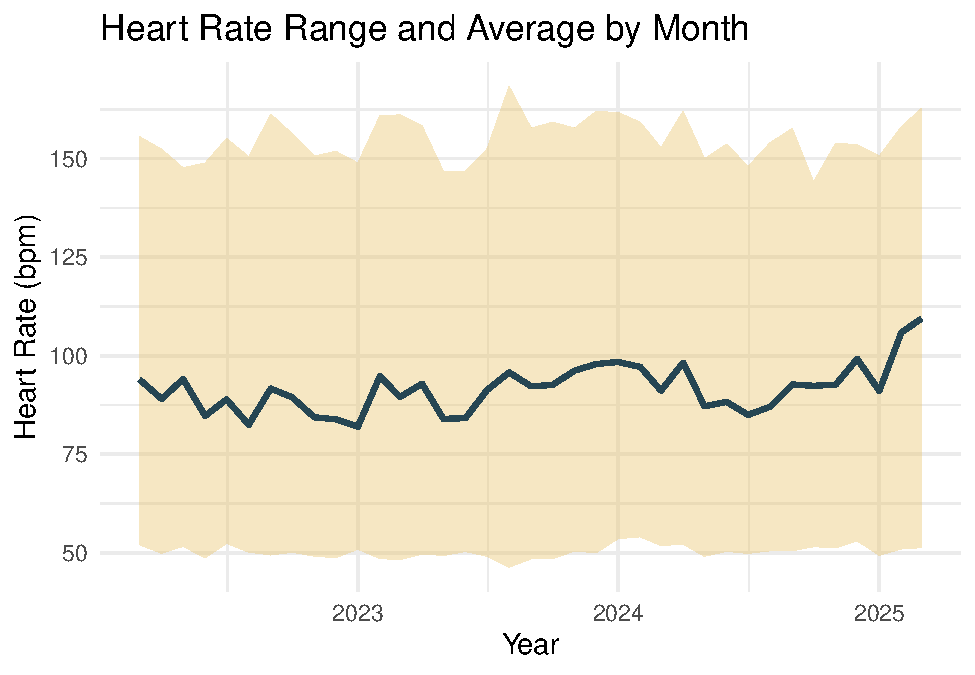
\includegraphics{analysis_files/figure-latex/unnamed-chunk-5-1.pdf}

\subsubsection{Times Ran and Walked Across
Time}\label{times-ran-and-walked-across-time}

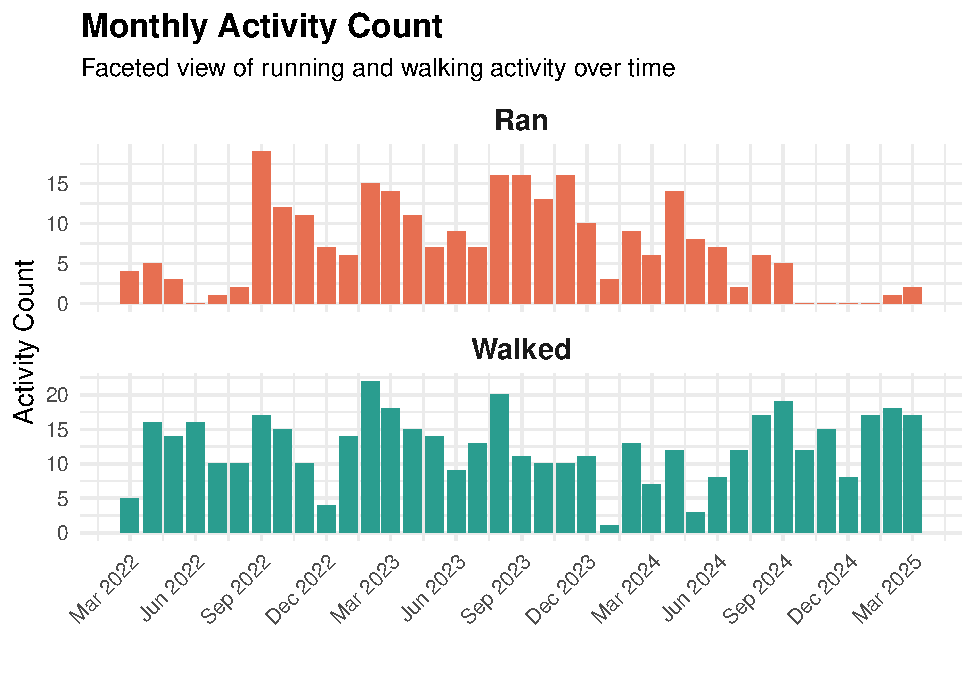
\includegraphics{analysis_files/figure-latex/unnamed-chunk-6-1.pdf}

\subsubsection{Number of days each goal was achieved per
month}\label{number-of-days-each-goal-was-achieved-per-month}

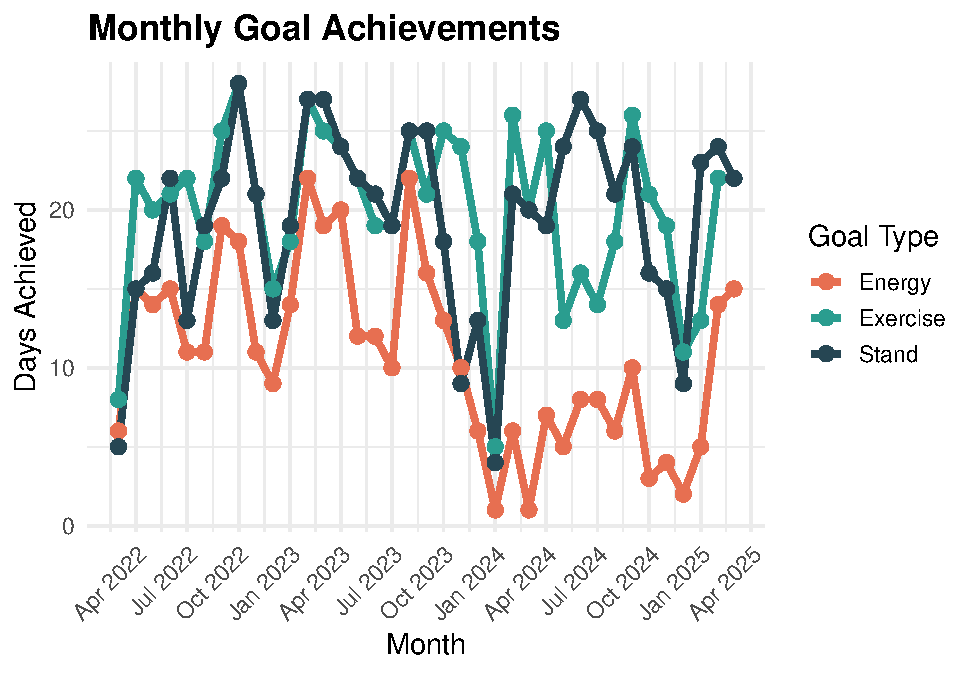
\includegraphics{analysis_files/figure-latex/unnamed-chunk-7-1.pdf}

\section{Analaysis 1: Did I work out that
day?}\label{analaysis-1-did-i-work-out-that-day}

\subsubsection{Poisson (Predicting Count of Workout Days Across Months)
Vs. Linear
Model}\label{poisson-predicting-count-of-workout-days-across-months-vs.-linear-model}

The Poisson (red) and linear (purple) lines are nearly identical across
all three heart rate types. Because the Poisson line closely follows the
linear regression line, we can conclude:

\begin{itemize}
\tightlist
\item
  The relationship between heart rate and workout count is well captured
  using a Poisson model, which is statistically more appropriate for
  counts.
\item
  There's no major non-linearity or overdispersion visible that would
  make the Poisson model clearly inferior or inappropriate.
\end{itemize}

\begin{Shaded}
\begin{Highlighting}[]
\NormalTok{low\_model }\OtherTok{\textless{}{-}} \FunctionTok{glm}\NormalTok{(num\_worked\_out }\SpecialCharTok{\textasciitilde{}}\NormalTok{ low\_heart\_rate, }\AttributeTok{family =} \FunctionTok{poisson}\NormalTok{(}\AttributeTok{link =} \StringTok{"log"}\NormalTok{), }
                 \AttributeTok{data =}\NormalTok{ parsed\_monthly\_summary)}
\NormalTok{high\_model }\OtherTok{\textless{}{-}} \FunctionTok{glm}\NormalTok{(num\_worked\_out }\SpecialCharTok{\textasciitilde{}}\NormalTok{ high\_heart\_rate, }\AttributeTok{family =} \FunctionTok{poisson}\NormalTok{(}\AttributeTok{link =} \StringTok{"log"}\NormalTok{), }
                  \AttributeTok{data =}\NormalTok{ parsed\_monthly\_summary)}
\NormalTok{avg\_model }\OtherTok{\textless{}{-}} \FunctionTok{glm}\NormalTok{(num\_worked\_out }\SpecialCharTok{\textasciitilde{}}\NormalTok{ avg\_heart\_rate, }\AttributeTok{family =} \FunctionTok{poisson}\NormalTok{(}\AttributeTok{link =} \StringTok{"log"}\NormalTok{), }
                 \AttributeTok{data =}\NormalTok{ parsed\_monthly\_summary)}

\NormalTok{low\_lm\_model }\OtherTok{\textless{}{-}} \FunctionTok{lm}\NormalTok{(num\_worked\_out }\SpecialCharTok{\textasciitilde{}}\NormalTok{ low\_heart\_rate, }\AttributeTok{data =}\NormalTok{ parsed\_monthly\_summary)}
\NormalTok{high\_lm\_model }\OtherTok{\textless{}{-}} \FunctionTok{lm}\NormalTok{(num\_worked\_out }\SpecialCharTok{\textasciitilde{}}\NormalTok{ high\_heart\_rate, }\AttributeTok{data =}\NormalTok{ parsed\_monthly\_summary)}
\NormalTok{avg\_lm\_model }\OtherTok{\textless{}{-}} \FunctionTok{lm}\NormalTok{(num\_worked\_out }\SpecialCharTok{\textasciitilde{}}\NormalTok{ avg\_heart\_rate, }\AttributeTok{data =}\NormalTok{ parsed\_monthly\_summary)}
\end{Highlighting}
\end{Shaded}

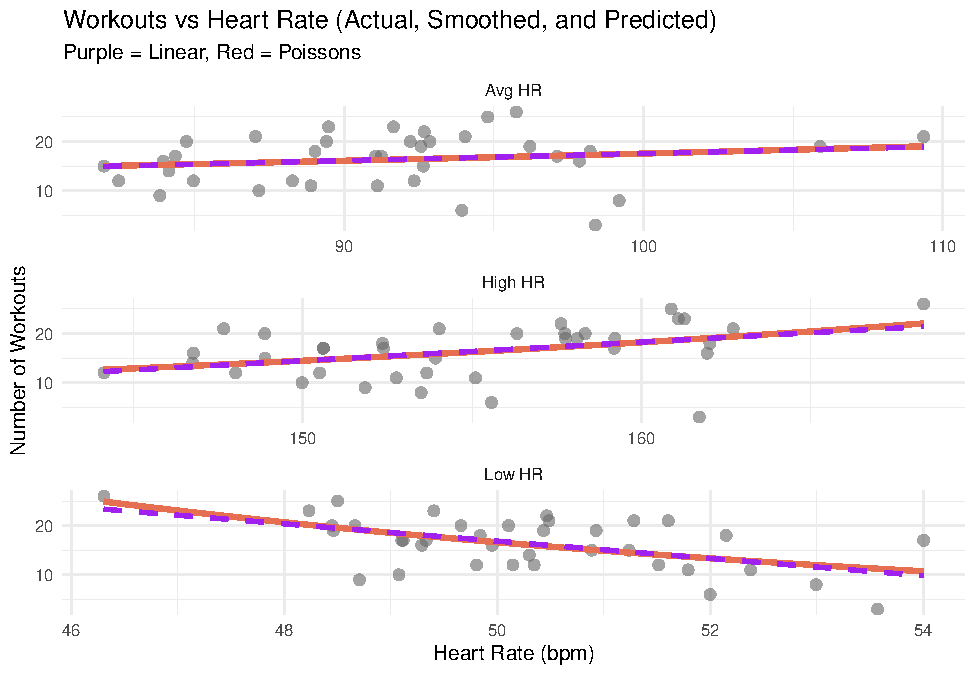
\includegraphics{analysis_files/figure-latex/unnamed-chunk-9-1.pdf}

\subsubsection{Tests}\label{tests}

\begin{longtable}[]{@{}
  >{\raggedright\arraybackslash}p{(\columnwidth - 12\tabcolsep) * \real{0.1212}}
  >{\raggedleft\arraybackslash}p{(\columnwidth - 12\tabcolsep) * \real{0.1061}}
  >{\raggedleft\arraybackslash}p{(\columnwidth - 12\tabcolsep) * \real{0.0909}}
  >{\raggedleft\arraybackslash}p{(\columnwidth - 12\tabcolsep) * \real{0.1212}}
  >{\raggedleft\arraybackslash}p{(\columnwidth - 12\tabcolsep) * \real{0.1515}}
  >{\raggedleft\arraybackslash}p{(\columnwidth - 12\tabcolsep) * \real{0.1212}}
  >{\raggedleft\arraybackslash}p{(\columnwidth - 12\tabcolsep) * \real{0.2879}}@{}}
\caption{Model Summary Table}\tabularnewline
\toprule\noalign{}
\begin{minipage}[b]{\linewidth}\raggedright
model
\end{minipage} & \begin{minipage}[b]{\linewidth}\raggedleft
beta
\end{minipage} & \begin{minipage}[b]{\linewidth}\raggedleft
SE
\end{minipage} & \begin{minipage}[b]{\linewidth}\raggedleft
z\_score
\end{minipage} & \begin{minipage}[b]{\linewidth}\raggedleft
z\_squared
\end{minipage} & \begin{minipage}[b]{\linewidth}\raggedleft
p\_value
\end{minipage} & \begin{minipage}[b]{\linewidth}\raggedleft
deviance\_explained
\end{minipage} \\
\midrule\noalign{}
\endfirsthead
\toprule\noalign{}
\begin{minipage}[b]{\linewidth}\raggedright
model
\end{minipage} & \begin{minipage}[b]{\linewidth}\raggedleft
beta
\end{minipage} & \begin{minipage}[b]{\linewidth}\raggedleft
SE
\end{minipage} & \begin{minipage}[b]{\linewidth}\raggedleft
z\_score
\end{minipage} & \begin{minipage}[b]{\linewidth}\raggedleft
z\_squared
\end{minipage} & \begin{minipage}[b]{\linewidth}\raggedleft
p\_value
\end{minipage} & \begin{minipage}[b]{\linewidth}\raggedleft
deviance\_explained
\end{minipage} \\
\midrule\noalign{}
\endhead
\bottomrule\noalign{}
\endlastfoot
Low HR & -0.109 & 0.026 & 4.213 & 17.751 & 0.00003 & 17.951 \\
High HR & 0.023 & 0.007 & 3.127 & 9.780 & 0.00176 & 9.742 \\
Avg HR & 0.009 & 0.007 & 1.320 & 1.743 & 0.18673 & 1.722 \\
\end{longtable}

\paragraph{Interpretation of Results}\label{interpretation-of-results}

So\ldots{}

Low Heart Rate (Resting HR)

\begin{itemize}
\tightlist
\item
  Strongest predictor (highest z, lowest p-value, most deviance
  explained)
\item
  Negative beta = Lower resting HR is associated with more workouts
\item
  A 1 bpm decrease in resting HR increases expected workouts by
  \textasciitilde10\% (e\^{}-0.109 ≈ 0.897 = \textasciitilde10\%
  reduction in workouts per 1 bpm increase)
\end{itemize}

High HR adds value but to a lesser degree.

\begin{itemize}
\tightlist
\item
  Also significant (p \textasciitilde{} .0018)
\item
  Positive beta = Higher peak HR is associated with more workouts
\item
  Each 1 bpm increase in high HR predicts a \textasciitilde2.3\%
  increase in workout days.
\end{itemize}

Average Heart Rate

\begin{itemize}
\tightlist
\item
  Not significant (p = 0.187)
\item
  Possibly too noisy or generic a measure to reflect true activity
  behavior
\end{itemize}

\subsubsection{Logistic Binary (Predicting Whether I Worked Out on a
Given
Day)}\label{logistic-binary-predicting-whether-i-worked-out-on-a-given-day}

\begin{Shaded}
\begin{Highlighting}[]
\NormalTok{low\_model }\OtherTok{\textless{}{-}} \FunctionTok{glm}\NormalTok{(worked\_out }\SpecialCharTok{\textasciitilde{}}\NormalTok{ low\_heart\_rate, }\AttributeTok{family =} \FunctionTok{binomial}\NormalTok{(), }\AttributeTok{data =}\NormalTok{ parsed\_clean\_by\_day)}
\NormalTok{high\_model }\OtherTok{\textless{}{-}} \FunctionTok{glm}\NormalTok{(worked\_out }\SpecialCharTok{\textasciitilde{}}\NormalTok{ high\_heart\_rate, }\AttributeTok{family =} \FunctionTok{binomial}\NormalTok{(), }\AttributeTok{data =}\NormalTok{ parsed\_clean\_by\_day)}
\NormalTok{avg\_model }\OtherTok{\textless{}{-}} \FunctionTok{glm}\NormalTok{(worked\_out }\SpecialCharTok{\textasciitilde{}}\NormalTok{ day\_avg\_heart\_rate, }\AttributeTok{family =} \FunctionTok{binomial}\NormalTok{(), }\AttributeTok{data =}\NormalTok{ parsed\_clean\_by\_day)}
\end{Highlighting}
\end{Shaded}

\begin{longtable}[]{@{}lrrrrr@{}}
\toprule\noalign{}
model & beta & SE & z\_score & p\_value & odds\_ratio \\
\midrule\noalign{}
\endhead
\bottomrule\noalign{}
\endlastfoot
Low HR & 0.011 & 0.015 & 0.730 & 0.46538 & 1.011 \\
High HR & 0.054 & 0.004 & 14.512 & 0.00000 & 1.056 \\
Avg HR & 0.090 & 0.006 & 14.108 & 0.00000 & 1.094 \\
\end{longtable}

Average Heart Rate

\begin{itemize}
\tightlist
\item
  Has the strongest effect on predicting workout likelihood.
\item
  Every 1 bpm increase in avg HR is associated with a 9.4\% increase in
  the odds of having worked out that day.
\item
  Highly statistically significant (p \textless{} 0.0001), indicating a
  robust relationship.
\end{itemize}

High Heart Rate

\begin{itemize}
\tightlist
\item
  Also a significant predictor.
\item
  Every 1 bpm increase in high HR increases the odds of working out by
  5.6\%.
\item
  Likely reflects workout intensity -- a higher max HR is a strong
  indicator that I engaged in physical effort.
\end{itemize}

Low Heart Rate

\begin{itemize}
\tightlist
\item
  Not statistically significant (p = 0.465).
\item
  Small beta (0.011) and an odds ratio close to 1 suggest no reliable
  link between low HR (resting) and working out on that specific day.
\item
  May be more useful for modeling long-term fitness, rather than
  day-level behavior.
\end{itemize}

\section{Analaysis 2: Seasons}\label{analaysis-2-seasons}

\subsection{Count of Workouts per
Month}\label{count-of-workouts-per-month}

This boxplot shows how my monthly workout counts vary across seasons,
summarizing data over multiple years.

\begin{longtable}[]{@{}lll@{}}
\caption{Summary of Workout Behavior by Season}\tabularnewline
\toprule\noalign{}
Season & Activity Level & Notes \\
\midrule\noalign{}
\endfirsthead
\toprule\noalign{}
Season & Activity Level & Notes \\
\midrule\noalign{}
\endhead
\bottomrule\noalign{}
\endlastfoot
Spring & High \& consistent & Strong, steady routine \\
Summer & Variable & Some very active, some low months \\
Fall & High \& consistent & Likely a return to routine \\
Winter & Lower & Less frequent workouts, higher drop-off \\
\end{longtable}

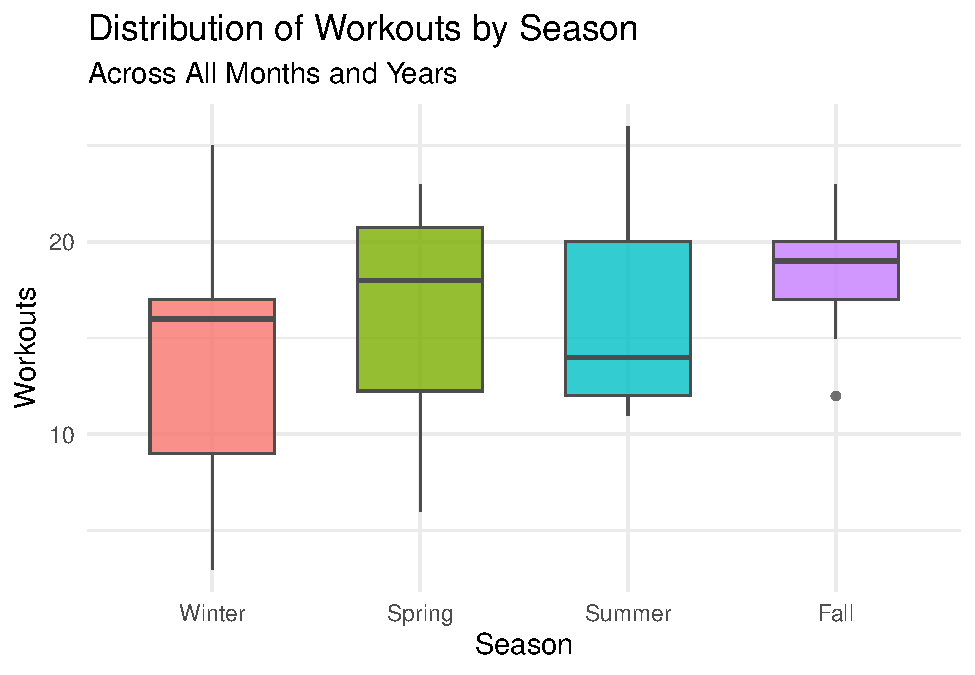
\includegraphics{analysis_files/figure-latex/unnamed-chunk-14-1.pdf}

\subsection{Poisson Regression: Can It Predict My Monthly Workout
Count\ldots{} Based on
Season?}\label{poisson-regression-can-it-predict-my-monthly-workout-count-based-on-season}

\begin{Shaded}
\begin{Highlighting}[]
\NormalTok{poisson\_season\_model }\OtherTok{\textless{}{-}} \FunctionTok{glm}\NormalTok{(}
\NormalTok{  num\_worked\_out }\SpecialCharTok{\textasciitilde{}}\NormalTok{ season,}
  \AttributeTok{data =}\NormalTok{ parsed\_monthly\_summary,}
  \AttributeTok{family =} \FunctionTok{poisson}\NormalTok{(}\AttributeTok{link =} \StringTok{"log"}\NormalTok{)}
\NormalTok{)}

\CommentTok{\# summary(poisson\_season\_model)}
\end{Highlighting}
\end{Shaded}

\begin{longtable}[]{@{}
  >{\raggedright\arraybackslash}p{(\columnwidth - 6\tabcolsep) * \real{0.0671}}
  >{\raggedleft\arraybackslash}p{(\columnwidth - 6\tabcolsep) * \real{0.0604}}
  >{\raggedright\arraybackslash}p{(\columnwidth - 6\tabcolsep) * \real{0.0537}}
  >{\raggedright\arraybackslash}p{(\columnwidth - 6\tabcolsep) * \real{0.8188}}@{}}
\caption{Coefficients Table: Poisson Regression of Workouts by
Season}\tabularnewline
\toprule\noalign{}
\begin{minipage}[b]{\linewidth}\raggedright
Term
\end{minipage} & \begin{minipage}[b]{\linewidth}\raggedleft
Estimate
\end{minipage} & \begin{minipage}[b]{\linewidth}\raggedright
p-value
\end{minipage} & \begin{minipage}[b]{\linewidth}\raggedright
Interpretation
\end{minipage} \\
\midrule\noalign{}
\endfirsthead
\toprule\noalign{}
\begin{minipage}[b]{\linewidth}\raggedright
Term
\end{minipage} & \begin{minipage}[b]{\linewidth}\raggedleft
Estimate
\end{minipage} & \begin{minipage}[b]{\linewidth}\raggedright
p-value
\end{minipage} & \begin{minipage}[b]{\linewidth}\raggedright
Interpretation
\end{minipage} \\
\midrule\noalign{}
\endhead
\bottomrule\noalign{}
\endlastfoot
Intercept & 2.66259 & \textless{} 0.001 & Baseline: Winter. Exp(2.66)
\textasciitilde{} 14.3 workouts/month in winter. \\
Spring & 0.13469 & 0.252 & Not statistically significant. Spring may
slightly increase workouts, but we're not confident. \\
Summer & 0.11692 & 0.334 & Also not significant. Summer doesn't strongly
differ from winter in workout counts. \\
Fall & 0.25818 & 0.028 & Statistically significant! Fall months have
higher workout counts compared to winter (about 29\% more, exp(0.258)
\textasciitilde{} 1.29). \\
\end{longtable}

\paragraph{Model Fit}\label{model-fit}

\begin{itemize}
\tightlist
\item
  Null deviance: 70.58
\item
  Residual deviance: 65.65
\item
  Chi-squared test p-value: 0.1766
\end{itemize}

This means that while fall stands out, season overall is not a strong
predictor of workout count across all months and years.

\subsection{Logistic Regression --- Daily Probability of Working
Out}\label{logistic-regression-daily-probability-of-working-out}

\begin{Shaded}
\begin{Highlighting}[]
\CommentTok{\# Binary outcome: worked out or not}
\NormalTok{logit\_season\_model }\OtherTok{\textless{}{-}} \FunctionTok{glm}\NormalTok{(}
\NormalTok{  worked\_out }\SpecialCharTok{\textasciitilde{}}\NormalTok{ season,}
  \AttributeTok{data =}\NormalTok{ parsed\_clean\_by\_day,}
  \AttributeTok{family =} \FunctionTok{binomial}\NormalTok{()}
\NormalTok{)}
\end{Highlighting}
\end{Shaded}

\begin{longtable}[]{@{}
  >{\raggedright\arraybackslash}p{(\columnwidth - 6\tabcolsep) * \real{0.1377}}
  >{\raggedleft\arraybackslash}p{(\columnwidth - 6\tabcolsep) * \real{0.0652}}
  >{\raggedleft\arraybackslash}p{(\columnwidth - 6\tabcolsep) * \real{0.0580}}
  >{\raggedright\arraybackslash}p{(\columnwidth - 6\tabcolsep) * \real{0.7391}}@{}}
\caption{Logistic Regression Coefficients: Predicting Daily Workout from
Season}\tabularnewline
\toprule\noalign{}
\begin{minipage}[b]{\linewidth}\raggedright
Term
\end{minipage} & \begin{minipage}[b]{\linewidth}\raggedleft
Estimate
\end{minipage} & \begin{minipage}[b]{\linewidth}\raggedleft
p-value
\end{minipage} & \begin{minipage}[b]{\linewidth}\raggedright
Interpretation
\end{minipage} \\
\midrule\noalign{}
\endfirsthead
\toprule\noalign{}
\begin{minipage}[b]{\linewidth}\raggedright
Term
\end{minipage} & \begin{minipage}[b]{\linewidth}\raggedleft
Estimate
\end{minipage} & \begin{minipage}[b]{\linewidth}\raggedleft
p-value
\end{minipage} & \begin{minipage}[b]{\linewidth}\raggedright
Interpretation
\end{minipage} \\
\midrule\noalign{}
\endhead
\bottomrule\noalign{}
\endlastfoot
Intercept (Winter) & 0.46536 & 0.001 & Winter is the baseline. Converts
to \textasciitilde61\% chance of working out (exp(0.465)/(1 +
exp(0.465)) ≈ 0.614). \\
Spring & -0.06598 & 0.725 & Not significant. Slightly lower odds of
working out vs.~winter. \\
Summer & -0.27612 & 0.142 & Also not significant. Suggests decreased
odds, but we can't confidently say so. \\
Fall & 0.03751 & 0.843 & Nearly no effect, and not statistically
significant. \\
\end{longtable}

\paragraph{Chi-squared test (ANOVA):}\label{chi-squared-test-anova}

The p = 0.2938 indicate that season as a whole does not significantly
improve model fit.

\begin{Shaded}
\begin{Highlighting}[]
\CommentTok{\# anova(logit\_season\_model)}
\end{Highlighting}
\end{Shaded}

\paragraph{Visualize}\label{visualize}

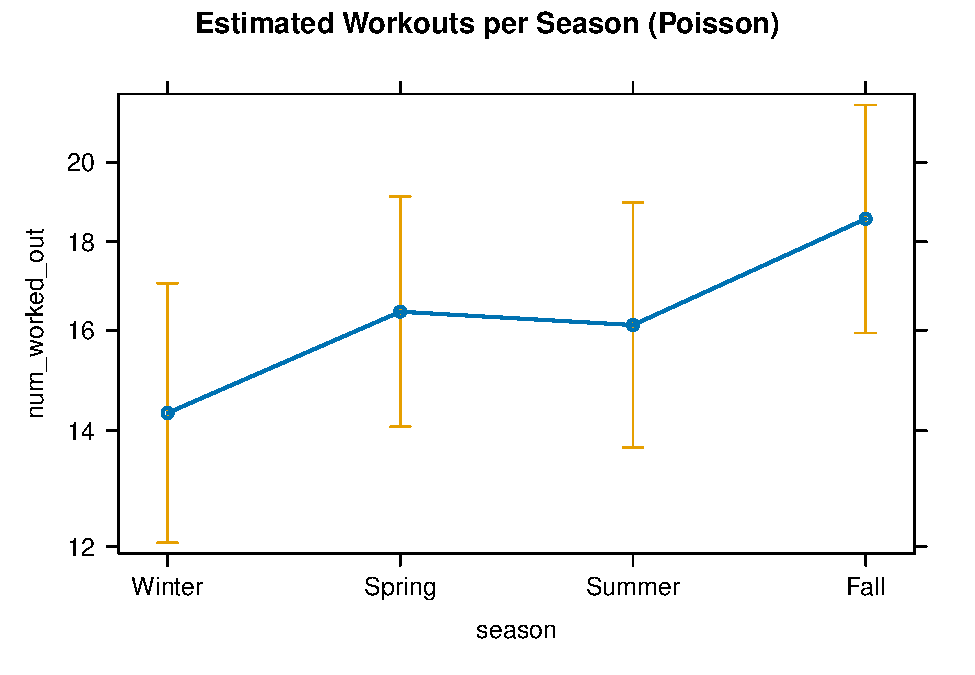
\includegraphics{analysis_files/figure-latex/unnamed-chunk-21-1.pdf}
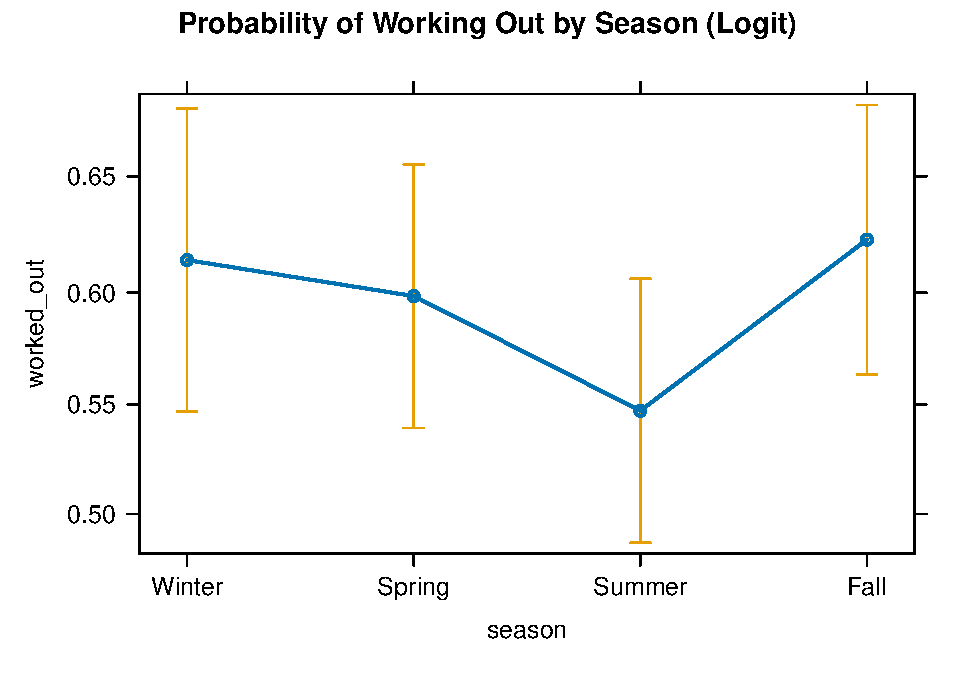
\includegraphics{analysis_files/figure-latex/unnamed-chunk-21-2.pdf}

\section{Consistency Score - Goals
Meet}\label{consistency-score---goals-meet}

\subsubsection{Trifecta Days as Count Outcome (Poisson Regression) --
Monthly}\label{trifecta-days-as-count-outcome-poisson-regression-monthly}

Conclusion: I am slightly more likely to hit my trifecta goals in summer
(with a potential \textasciitilde31\% increase), but the effect of
season overall isn't statistically strong. Winter remains my base with
\textasciitilde8 trifecta days/month.

\begin{Shaded}
\begin{Highlighting}[]
\NormalTok{glm\_trifecta }\OtherTok{\textless{}{-}} \FunctionTok{glm}\NormalTok{(num\_trifecta\_days }\SpecialCharTok{\textasciitilde{}}\NormalTok{ season, }\AttributeTok{data =}\NormalTok{ monthly\_consistency, }\AttributeTok{family =} \FunctionTok{poisson}\NormalTok{())}
\CommentTok{\#summary(glm\_trifecta)}
\end{Highlighting}
\end{Shaded}

\begin{longtable}[]{@{}
  >{\raggedright\arraybackslash}p{(\columnwidth - 6\tabcolsep) * \real{0.1242}}
  >{\raggedleft\arraybackslash}p{(\columnwidth - 6\tabcolsep) * \real{0.0588}}
  >{\raggedright\arraybackslash}p{(\columnwidth - 6\tabcolsep) * \real{0.0523}}
  >{\raggedright\arraybackslash}p{(\columnwidth - 6\tabcolsep) * \real{0.7647}}@{}}
\caption{Poisson Regression: Predicting Trifecta Days by
Season}\tabularnewline
\toprule\noalign{}
\begin{minipage}[b]{\linewidth}\raggedright
Term
\end{minipage} & \begin{minipage}[b]{\linewidth}\raggedleft
Estimate
\end{minipage} & \begin{minipage}[b]{\linewidth}\raggedright
p-value
\end{minipage} & \begin{minipage}[b]{\linewidth}\raggedright
Interpretation
\end{minipage} \\
\midrule\noalign{}
\endfirsthead
\toprule\noalign{}
\begin{minipage}[b]{\linewidth}\raggedright
Term
\end{minipage} & \begin{minipage}[b]{\linewidth}\raggedleft
Estimate
\end{minipage} & \begin{minipage}[b]{\linewidth}\raggedright
p-value
\end{minipage} & \begin{minipage}[b]{\linewidth}\raggedright
Interpretation
\end{minipage} \\
\midrule\noalign{}
\endhead
\bottomrule\noalign{}
\endlastfoot
Intercept (Winter) & 2.0655 & \textless{} 0.001 & Baseline (Winter): On
average, \textasciitilde7.88 trifecta days/month in winter.
--\textgreater{} exp(2.0655) ≈ 7.88 \\
Spring & 0.2471 & 0.111 & Not statistically significant. Spring may
increase trifecta days by \textasciitilde28\% (exp(0.247)), but we can't
say confidently. \\
Summer & 0.2699 & 0.087 & Marginally significant (p \textasciitilde{}
0.087). Could imply \textasciitilde31\% more trifecta days than winter
(exp(0.27) \textasciitilde{} 1.31). \\
Fall & 0.2482 & 0.117 & Similar to spring --- slight positive trend
(\textasciitilde28\% increase), but not statistically strong. \\
\end{longtable}

\subsection{Model Odds of ``Trifecta Day'' (logistic version) --
Daily}\label{model-odds-of-trifecta-day-logistic-version-daily}

Season has no significant influence on the likelihood of hitting a
trifecta day. I am about 1 in 3 likely to hit all 3 goals on any given
day in winter -- and that probability stays pretty stable across
seasons.

\begin{Shaded}
\begin{Highlighting}[]
\NormalTok{parsed\_clean\_by\_day }\OtherTok{\textless{}{-}}\NormalTok{ parsed\_clean\_by\_day }\SpecialCharTok{|\textgreater{}}
  \FunctionTok{mutate}\NormalTok{(}\AttributeTok{trifecta\_day =}\NormalTok{ activeEnergyGoalAchieved }\SpecialCharTok{\&}\NormalTok{ appleExerciseTimeGoalAchieved }\SpecialCharTok{\&}\NormalTok{ appleStandHoursGoalAchieved)}

\NormalTok{glm\_trifecta\_day }\OtherTok{\textless{}{-}} \FunctionTok{glm}\NormalTok{(trifecta\_day }\SpecialCharTok{\textasciitilde{}} \FunctionTok{factor}\NormalTok{(season), }\AttributeTok{data =}\NormalTok{ parsed\_clean\_by\_day, }\AttributeTok{family =} \FunctionTok{binomial}\NormalTok{())}
\end{Highlighting}
\end{Shaded}

\begin{longtable}[]{@{}
  >{\raggedright\arraybackslash}p{(\columnwidth - 6\tabcolsep) * \real{0.1301}}
  >{\raggedleft\arraybackslash}p{(\columnwidth - 6\tabcolsep) * \real{0.0616}}
  >{\raggedright\arraybackslash}p{(\columnwidth - 6\tabcolsep) * \real{0.0548}}
  >{\raggedright\arraybackslash}p{(\columnwidth - 6\tabcolsep) * \real{0.7534}}@{}}
\caption{Logistic Regression: Predicting Trifecta Days from
Season}\tabularnewline
\toprule\noalign{}
\begin{minipage}[b]{\linewidth}\raggedright
Term
\end{minipage} & \begin{minipage}[b]{\linewidth}\raggedleft
Estimate
\end{minipage} & \begin{minipage}[b]{\linewidth}\raggedright
p-value
\end{minipage} & \begin{minipage}[b]{\linewidth}\raggedright
Interpretation
\end{minipage} \\
\midrule\noalign{}
\endfirsthead
\toprule\noalign{}
\begin{minipage}[b]{\linewidth}\raggedright
Term
\end{minipage} & \begin{minipage}[b]{\linewidth}\raggedleft
Estimate
\end{minipage} & \begin{minipage}[b]{\linewidth}\raggedright
p-value
\end{minipage} & \begin{minipage}[b]{\linewidth}\raggedright
Interpretation
\end{minipage} \\
\midrule\noalign{}
\endhead
\bottomrule\noalign{}
\endlastfoot
Intercept (Winter) & -0.672 & \textless{} 0.001 & Winter is the
baseline. Converts to \textasciitilde33.8\% chance of a trifecta day:
exp(-0.672) / (1 + exp(-0.672)) ≈ 0.338. \\
Spring & 0.134 & 0.487 & Not significant. Small (non-reliable) increase
in odds vs.~winter. \\
Summer & 0.057 & 0.770 & No meaningful difference from winter. \\
Fall & 0.007 & 0.973 & Almost identical to winter --- essentially no
effect. \\
\end{longtable}

\section{Ran and Season}\label{ran-and-season}

This model estimates the likelihood of going for a run on a given day
using season as the predictor. Fall is my most reliably active season
for running, with a significant increase in the likelihood of going for
a run compared to winter. Spring and summer show no significant change,
but summer might actually suppress my running tendencies a bit.

\begin{Shaded}
\begin{Highlighting}[]
\NormalTok{ran\_season }\OtherTok{\textless{}{-}} \FunctionTok{glm}\NormalTok{(ran }\SpecialCharTok{\textasciitilde{}} \FunctionTok{factor}\NormalTok{(season), }\AttributeTok{data =}\NormalTok{ parsed\_clean\_by\_day, }\AttributeTok{family =} \FunctionTok{binomial}\NormalTok{())}
\end{Highlighting}
\end{Shaded}

\begin{longtable}[]{@{}
  >{\raggedright\arraybackslash}p{(\columnwidth - 6\tabcolsep) * \real{0.1338}}
  >{\raggedleft\arraybackslash}p{(\columnwidth - 6\tabcolsep) * \real{0.0634}}
  >{\raggedright\arraybackslash}p{(\columnwidth - 6\tabcolsep) * \real{0.0563}}
  >{\raggedright\arraybackslash}p{(\columnwidth - 6\tabcolsep) * \real{0.7465}}@{}}
\caption{Logistic Regression: Predicting Running Behavior by
Season}\tabularnewline
\toprule\noalign{}
\begin{minipage}[b]{\linewidth}\raggedright
Term
\end{minipage} & \begin{minipage}[b]{\linewidth}\raggedleft
Estimate
\end{minipage} & \begin{minipage}[b]{\linewidth}\raggedright
p-value
\end{minipage} & \begin{minipage}[b]{\linewidth}\raggedright
Interpretation
\end{minipage} \\
\midrule\noalign{}
\endfirsthead
\toprule\noalign{}
\begin{minipage}[b]{\linewidth}\raggedright
Term
\end{minipage} & \begin{minipage}[b]{\linewidth}\raggedleft
Estimate
\end{minipage} & \begin{minipage}[b]{\linewidth}\raggedright
p-value
\end{minipage} & \begin{minipage}[b]{\linewidth}\raggedright
Interpretation
\end{minipage} \\
\midrule\noalign{}
\endhead
\bottomrule\noalign{}
\endlastfoot
Intercept (Winter) & -1.1371 & \textless{} 0.001 & Winter is the
baseline. This converts to a 24.2\% chance of running:
exp(-1.1371)/(1+exp(-1.1371)) ≈ 0.242 \\
Spring & 0.1428 & 0.498 & Not significant. Slight increase in odds
vs.~winter, but not reliable. \\
Summer & -0.3215 & 0.153 & Not significant, but suggests lower odds of
running in summer vs.~winter. \\
Fall & 0.4884 & 0.018 & Statistically significant. Fall has 63\% higher
odds of running compared to winter. (exp(0.4884) ≈ 1.63) \\
\end{longtable}

\subparagraph{Model Fit Summary}\label{model-fit-summary}

\begin{itemize}
\tightlist
\item
  Null deviance: 1171.0
\item
  Residual deviance: 1153.9
\item
  AIC: 1161.9 Season explains some variance in running behavior ---
  particularly due to Fall's significance
\end{itemize}

\section{Brute Force Athlete Heart Rate
ROC}\label{brute-force-athlete-heart-rate-roc}

Exhaustive AUC Comparison of Predictor Combinations for is\_athlete
Classification

\texttt{is\_athlete} Variable

\begin{itemize}
\item
  is\_athlete = TRUE --\textgreater{} My lowest recorded heart rate for
  the day was between 40 and 60 bpm, which is a common physiological
  range for trained athletes.
\item
  is\_athlete = FALSE --\textgreater{} My lowest heart rate fell outside
  that range (either below 40 or above 60 bpm), so they likely don't
  exhibit resting HR levels consistent with trained athletes.
\end{itemize}

This script performs automated model selection by:

\begin{itemize}
\tightlist
\item
  Testing all combinations of predictors (1 to 6 variables at a time).
\item
  Fitting a logistic regression model to predict whether a day belongs
  to an ``athlete'' heart rate profile.
\item
  Evaluating each model's predictive performance using AUC (Area Under
  the ROC Curve).
\item
  Returning a sorted table of models ranked by their AUC.
\end{itemize}

Why AUC?

\begin{itemize}
\tightlist
\item
  AUC reflects how well the model distinguishes between classes
  (is\_athlete = TRUE/FALSE).
\item
  AUC of 1.0 = perfect model, 0.5 = random guessing.
\item
  Higher AUC = better classification performance.
\end{itemize}

Conclusion

The most predictive combination of whether I exhibit ``athlete-like
heart rate patterns'' includes stand hours, walking, running, and
seasonal context with it AUCs reaching 0.803, which indicates very
strong predictive power for a binary classification model in health
behavior.

\begin{Shaded}
\begin{Highlighting}[]
\NormalTok{parsed\_clean\_by\_day }\OtherTok{\textless{}{-}}\NormalTok{ parsed\_clean\_by\_day }\SpecialCharTok{|\textgreater{}}
  \FunctionTok{mutate}\NormalTok{(}\AttributeTok{is\_athlete =}\NormalTok{ low\_heart\_rate }\SpecialCharTok{\textgreater{}=} \DecValTok{40} \SpecialCharTok{\&}\NormalTok{ low\_heart\_rate }\SpecialCharTok{\textless{}=} \DecValTok{60}\NormalTok{)}

\CommentTok{\# define predictors}
\NormalTok{predictors }\OtherTok{\textless{}{-}} \FunctionTok{c}\NormalTok{(}\StringTok{"factor(season)"}\NormalTok{, }\StringTok{"EnergyBurned"}\NormalTok{, }\StringTok{"ExerciseTime"}\NormalTok{, }\StringTok{"standHours"}\NormalTok{, }\StringTok{"ran"}\NormalTok{, }\StringTok{"walk"}\NormalTok{)}

\CommentTok{\# all combinations of predictors (excluding empty set)}
\NormalTok{predictor\_combos }\OtherTok{\textless{}{-}} \FunctionTok{unlist}\NormalTok{(}\FunctionTok{lapply}\NormalTok{(}\DecValTok{1}\SpecialCharTok{:}\FunctionTok{length}\NormalTok{(predictors), }\ControlFlowTok{function}\NormalTok{(n) \{}
  \FunctionTok{combn}\NormalTok{(predictors, n, }\AttributeTok{simplify =} \ConstantTok{FALSE}\NormalTok{)}
\NormalTok{\}), }\AttributeTok{recursive =} \ConstantTok{FALSE}\NormalTok{)}

\CommentTok{\# evaluate each model}
\NormalTok{combo\_results }\OtherTok{\textless{}{-}} \FunctionTok{map\_dfr}\NormalTok{(predictor\_combos, }\ControlFlowTok{function}\NormalTok{(vars) \{}
\NormalTok{  formula\_str }\OtherTok{\textless{}{-}} \FunctionTok{paste}\NormalTok{(}\StringTok{"factor(is\_athlete) \textasciitilde{}"}\NormalTok{, }\FunctionTok{paste}\NormalTok{(vars, }\AttributeTok{collapse =} \StringTok{" + "}\NormalTok{))}
\NormalTok{  model }\OtherTok{\textless{}{-}} \FunctionTok{glm}\NormalTok{(}\FunctionTok{as.formula}\NormalTok{(formula\_str), }\AttributeTok{data =}\NormalTok{ parsed\_clean\_by\_day, }\AttributeTok{family =} \FunctionTok{binomial}\NormalTok{())}
\NormalTok{  pred }\OtherTok{\textless{}{-}} \FunctionTok{predict}\NormalTok{(model, }\AttributeTok{type =} \StringTok{"response"}\NormalTok{)}
  
  \CommentTok{\# Clean NAs}
\NormalTok{  valid }\OtherTok{\textless{}{-}} \FunctionTok{complete.cases}\NormalTok{(pred, parsed\_clean\_by\_day}\SpecialCharTok{$}\NormalTok{is\_athlete)}
  
  \ControlFlowTok{if}\NormalTok{ (}\FunctionTok{length}\NormalTok{(}\FunctionTok{unique}\NormalTok{(parsed\_clean\_by\_day}\SpecialCharTok{$}\NormalTok{is\_athlete[valid])) }\SpecialCharTok{\textless{}} \DecValTok{2}\NormalTok{) \{}
    \FunctionTok{return}\NormalTok{(}\ConstantTok{NULL}\NormalTok{) }\CommentTok{\# skip if only one class is present}
\NormalTok{  \}}
  
\NormalTok{  roc\_obj }\OtherTok{\textless{}{-}} \FunctionTok{roc}\NormalTok{(parsed\_clean\_by\_day}\SpecialCharTok{$}\NormalTok{is\_athlete[valid], pred[valid])}
  \FunctionTok{tibble}\NormalTok{(}
    \AttributeTok{predictors =} \FunctionTok{paste}\NormalTok{(vars, }\AttributeTok{collapse =} \StringTok{" + "}\NormalTok{),}
    \AttributeTok{auc =} \FunctionTok{as.numeric}\NormalTok{(}\FunctionTok{auc}\NormalTok{(roc\_obj))}
\NormalTok{  )}
\NormalTok{\})}

\CommentTok{\# sort by best AUC}
\NormalTok{combo\_results }\OtherTok{\textless{}{-}}\NormalTok{ combo\_results }\SpecialCharTok{|\textgreater{}}
  \FunctionTok{arrange}\NormalTok{(}\FunctionTok{desc}\NormalTok{(auc))}

\NormalTok{combo\_results }\SpecialCharTok{|\textgreater{}} 
  \FunctionTok{head}\NormalTok{(}\DecValTok{5}\NormalTok{) }\SpecialCharTok{|\textgreater{}} 
  \FunctionTok{kable}\NormalTok{()}
\end{Highlighting}
\end{Shaded}

\begin{longtable}[]{@{}
  >{\raggedright\arraybackslash}p{(\columnwidth - 2\tabcolsep) * \real{0.8765}}
  >{\raggedleft\arraybackslash}p{(\columnwidth - 2\tabcolsep) * \real{0.1235}}@{}}
\toprule\noalign{}
\begin{minipage}[b]{\linewidth}\raggedright
predictors
\end{minipage} & \begin{minipage}[b]{\linewidth}\raggedleft
auc
\end{minipage} \\
\midrule\noalign{}
\endhead
\bottomrule\noalign{}
\endlastfoot
factor(season) + ExerciseTime + standHours + ran + walk & 0.8032106 \\
factor(season) + EnergyBurned + ExerciseTime + standHours + ran + walk &
0.8030793 \\
factor(season) + EnergyBurned + standHours + ran + walk & 0.8030356 \\
factor(season) + standHours + ran + walk & 0.8013297 \\
factor(season) + ExerciseTime + standHours + walk & 0.8010454 \\
\end{longtable}

\end{document}
